\begin{document}
	\chapter{Evaluation}
	\section{Success criteria} \label{Section: eval/success-criteria}
		blah
	\section{Features evaluation} \label{Section: eval/features}
		Even though the key module of the entire project was the one where the machine learning models are implemented, the set of features extracted for each node is at least as important because, without them being representative, the models will not be able to generalize well. For this reason, in this section, I will present the evaluation of the features I extracted for each node.
		
	\subsection{Feature importance algorithm} \label{Section: eval/features/alg}
		In order to measure the feature importance I made use of the Boruta algorithm, proposed by \textit{M. Kursa et al.}\cite{JSSv036i11}. It uses a random forest classification in order to compute the \textbf{z score} for every feature taken into consideration. 
		\\ \\
		In short, the algorithm is based on the same idea which forms the foundation of a random forest classifier, namely, that by adding randomness to the system and collecting results from the ensemble of randomized samples one can reduce the misleading impact of random fluctuations and correlations. In this case, this extra randomness provides a clearer view of which features really are important. The steps enumerated below are repeated until either the importance is assigned for all features or the algorithm has reached the previously set limit of random forests runs:
		\begin{enumerate}
			\item Extend the feature space by adding copies of all variables and then shuffle the added attributes in order to remove their correlations with the response.
			\item Run a random forest classifier on the extended dataset and gather the z-scores computed.
			\item Find the maximum z-score among the shadow features (MZSA) and assign a hit to every feature that scored better than MZSA
			\item For each feature with undetermined importance perform a two-sided equality test with MZSA
			\item Consider the features with importance significantly lower than MZSA as \textit{unimportant} and the ones with importance significantly higher than MZSA as \textit{important}.
			\item Remove all shadow attributes
		\end{enumerate}
	\subsection{Results \& discussion} \label{Section: eval/features/results}
		
	\section{Evaluation of machine learning models} \label{Section: eval/ml}
	\subsection{Evaluation methodology} \label{Section: eval/ml/methodology}
		In order to quantitatively evaluate the performance of the machine learning models implemented, I used a labelled dataset $\mathbf{s}$ containing $5,498$ nodes. Figure \ref{Fig: eval/ml/methodology/dist} shows how the labels and node types are distributed in the dataset used in this case. From there, we can observe that the node type distribution resembles the distribution that can be found in the general case in a provenance graph. Therefore, by evaluating the models on this dataset I can produce a comprehensive and accurate assessment of their performance. 
		\begin{figure}[H]
			\centering
			\begin{subfigure}{.4\textwidth}
				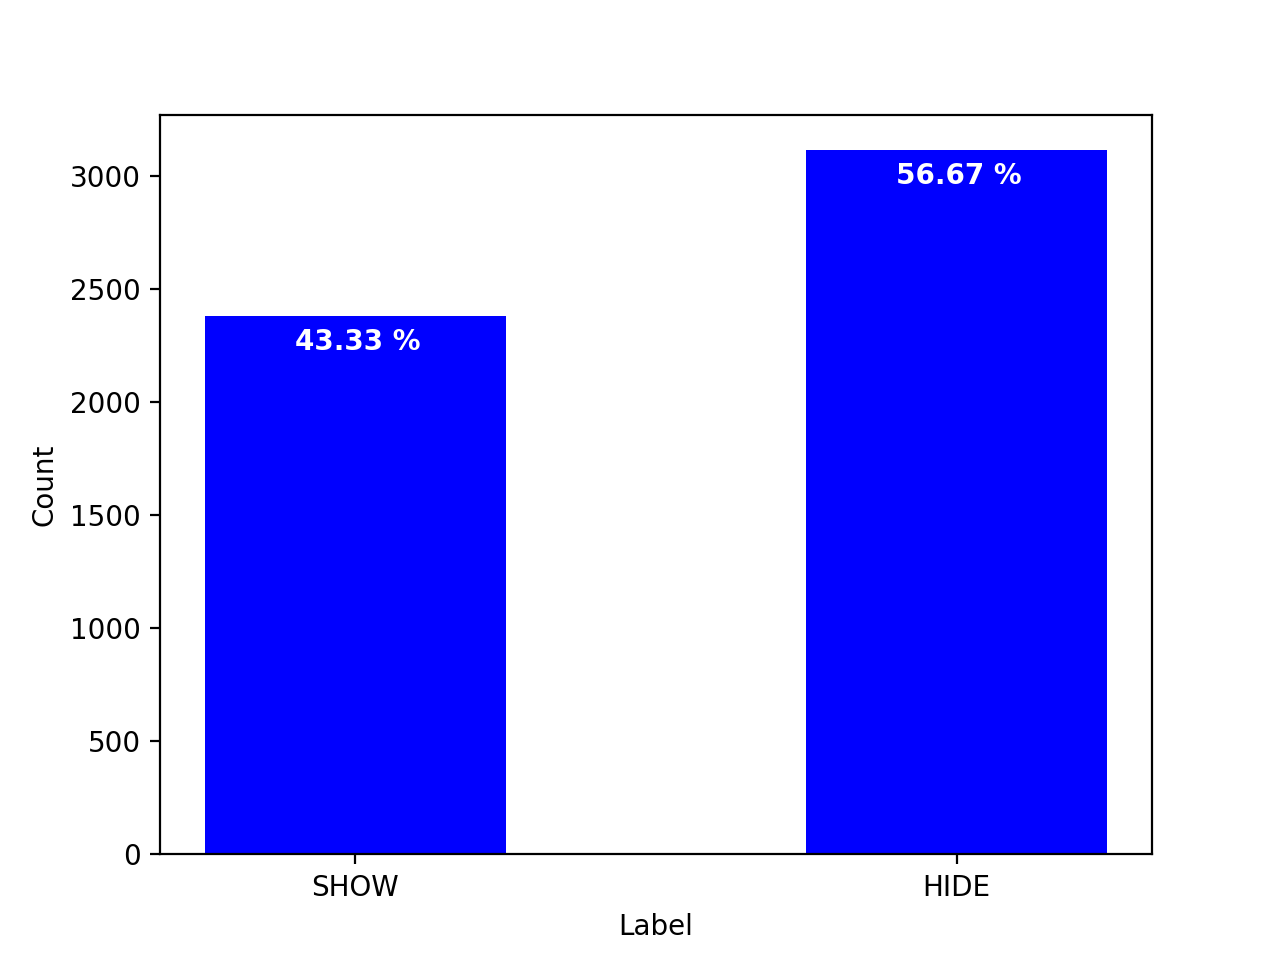
\includegraphics[width=\textwidth]{graphics/labels-dist}
			\end{subfigure}
			\hfill
			\begin{subfigure}{.4\textwidth}
				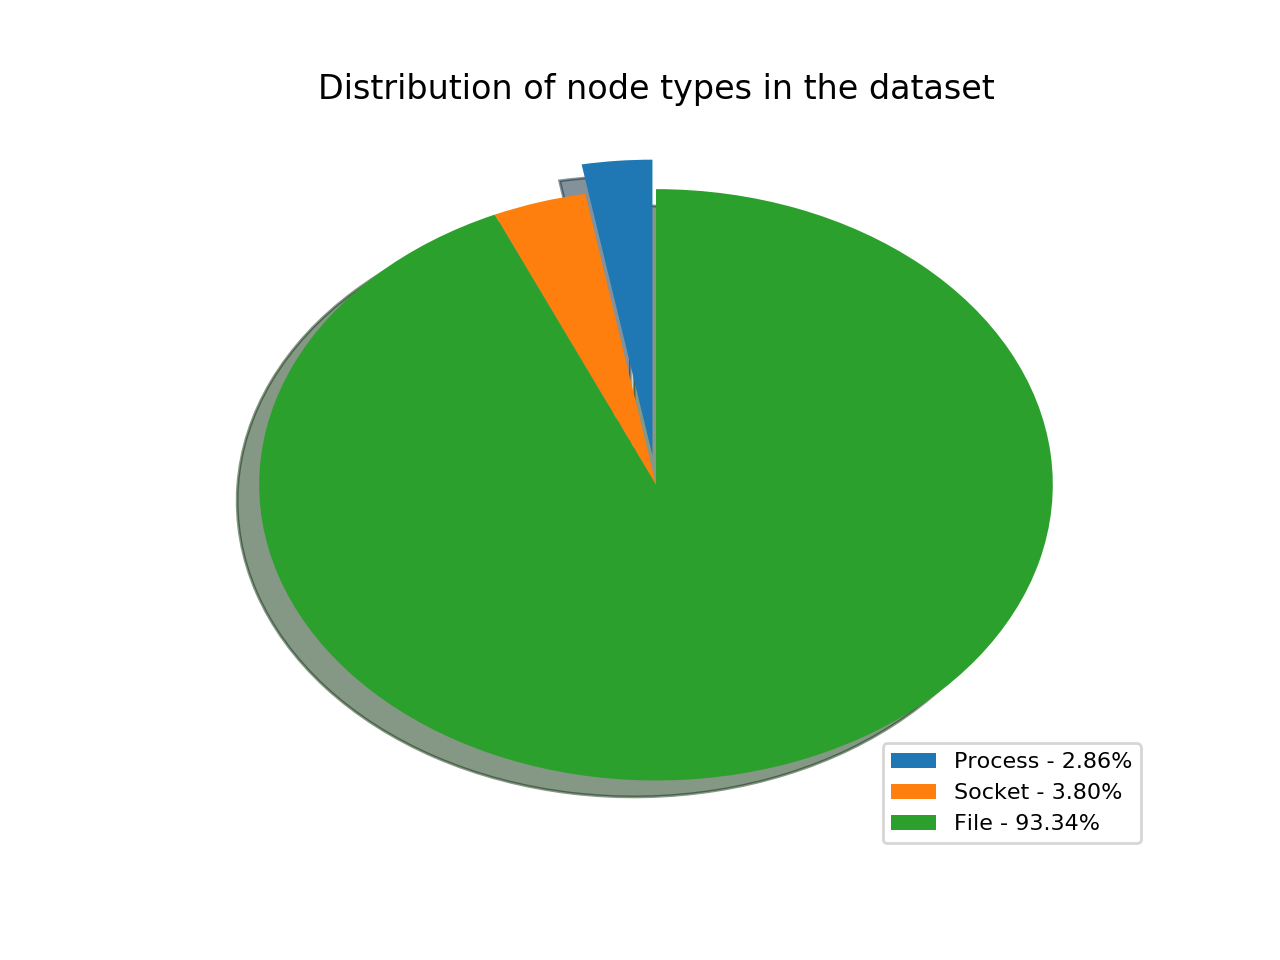
\includegraphics[width=\textwidth]{graphics/node-dist}
			\end{subfigure}
			\caption[Distributions of labels and node type in the dataset]{\textit{Left:} Distribution of the labels in the dataset. \textit{Right: }Distribution of the node types in the dataset.}
			\label{Fig: eval/ml/methodology/dist}
		\end{figure} 
		The technique used when evaluating the models was \textbf{k-fold cross validation}. Essentially, I split the dataset in $10$ equally-sized slots and use one at a time as a test set, while the other $9$ serve as the training set for the model. Figure \ref{Fig: impl/ml/methodology/kfold/first} shows how the dataset is divided in the first iteration of the cross-validation algorithm. For the models that require a validation set for optimising hyperparameters, the training set is split again in $10$ slots of equal sizes and uses one at a time as a validation set. This way, I ensure that none of the models is not tested on previously-seen examples and therefore I correctly evaluate how well they generalize on the given data.
		\begin{figure}[H]
			\centering
			\includegraphics[width=.8\textwidth]{graphics/k-fold}
			\caption{First step in k-fold cross validation}
			\label{Fig: impl/ml/methodology/kfold/first}
		\end{figure}
		
		At every iteration, I compute a set of metrics that for estimating the model's performance and the final result for every metric in part is given by averaging over the values obtained. 
	\subsection{Metrics involved} \label{Section: eval/ml/metrics}
	
		In this section, I will outline the metrics used when evaluating the machine learning models. The choice of good metrics is essential when comparatively evaluating a number of machine learning models. The simplest metric for evaluating of classification algorithms is \textbf{accuracy}, and can be computed using the formula: 
		\\
		\begin{equation}
			acc = \frac{\text{no. of correctly predicted nodes}}{\text{total no. of predicted nodes}}
		\end{equation}
		\\
		Accuracy, however, is not efficient when it comes to imbalanced data, as it is the case here(i.e. we have a $43\%/57\%$ \textit{SHOW/HIDE} distribution amongst the nodes). Therefore, more complex metrics are required in order to correctly assess the performance of the models implemented. These metrics are based on the notions of \textit{true positives, true negatives, false positives and false negatives}, which can easily be illustrated using a confusion matrix, such as the one from Figure \ref{Fig: eval/ml/metrics/confusion-matrix}.
		\begin{figure}[H]
			\centering
			\includegraphics[width=.7\textwidth]{graphics/confusion-matrix}
			\caption{Confusion matrix for two-class classification}
			\label{Fig: eval/ml/metrics/confusion-matrix}
		\end{figure}
		The metrics I used to evaluate the general performance of the models are presented in Table \ref{Table: eval/ml/metrics/metrics}. From those, the F1 score and the MCC are the most meaningful for this case, as they ignore the fact that the data is not balanced. The F1 score gives a value in the interval $[0, 1]$, with $1$ representing perfect prediction, while the MCC gives a value between $[-1, 1]$, where $1$ represents perfect prediction, $0$ not better than random and $-1$ a total disagreement between the predicted and true labels.
		\begin{longtable}{|p{.15\textwidth}|p{.40\textwidth}|c|}
		   \textbf{Metric} & \textbf{Intuition} &\textbf{Formula} \\
			\hline
			\textit{Precision} & fraction of nodes correctly labelled as \textit{SHOW} in all nodes classified. & {$\centering \text{precision} = \frac{tp}{tp+fp}$} \\
			\hline 
			\textit{Recall} & fraction of \textit{SHOW} nodes correctly classified. & $\text{recall} = \frac{tp}{tp+fn}$ \\
			\hline
			\textit{F1 score} & takes into consideration both the precision and the recall of the model in order to assess its performance & $\text{F1} = 2\times\frac{\text{precision}\times\text{recall}}{\text{precision} + \text{recall}}$\\
			\hline 
			\textit{Matthew's Correlation Coefficient (MCC)} & takes into account true and false positives and negatives in order to provide a balanced metric for the model's performance & $MCC = \frac{tp\times tn - fp\times fn}{\sqrt{(tp+fp)\times(tp+fn)\times(tn+fp)\times(tn+fn)}}$\\
			\hline
			\caption{Machine learning evaluation metrics}
			\label{Table: eval/ml/metrics/metrics}
		\end{longtable}
		
		\subsection{Results \& discussion} \label{Section: eval/ml/results}

		\section{Service time evaluation} \label{Section: eval/service-time}
			This project is meant to be a complete API that can be used in practice by the CADETS user interface. Therefore, besides the performance of the machine learning model used, it is essential to evaluate it in terms of the service speed as well. All the timing results were obtained using my personal machine. For a job processing $N$ nodes, the service time is calculated using the following formula:  
			\begin{equation}
				\text{service\_time} = N\times [CCT + CHR \times CET + (1-CHR) \times (CT + RCT)] + MLT
				\label{Eq: eval/service-time/overall}
			\end{equation}
			where: 
			\begin{itemize}
				\item $\mathbf{CCT} \in \mathbb{R}$ = Cache Check Time - time taking to check if a node is in the cache database and if the entry is still valid.
				\item $\mathbf{CHR} \in [0, 1]$ = Cache Hit Rate.
				\item $\textbf{CET} \in \mathbb{R}$ = Cache Extraction Time - time taking to extracted one cached result.
				\item $\textbf{CT} \in \mathbb{R}$ = Classification Time - time taking to classify a node. 
				\item $\textbf{RCT} \in \mathbb{R}$ = Result Caching Time - time required to add a new classification result to the cache database.
				\item $\mathbf{MLT} \in \mathbb{R}$ = Model Loading Time - time required to configure the model (i.e. defining its components and load the corresponding pre-optimised parameters)
			\end{itemize}
			In practice, the API is expected to re-use many of the classification results. For this reason, I assume the the cache to have a hit-rate $CHR = 90\%$. For simulation purposes, the database was populated with $10, 000$ nodes and $30$ completed jobs, each having processed $1, 000$ nodes. 
			\\ \\
			The first step performed by the application when the new job is initiated is to check the cache and try to get the nodes that are cached. In this given simulation environment, the Cache Check Time, Cache Extraction Time and Result Caching Time are $CCT=??????????$, $CET=???????????$ and $RCT=??????????????$, respectively.  
			
		\subsection{Classification timings} \label{Section: eval/service-time/classification}
			The classification time is not as straight-forward as the times shown so far. It was computed using the following formula:
			\begin{equation}
				CT = NTT + FET + MRT
			\end{equation}
			where: 
			\begin{itemize}
				\item $\mathbf{NTT} \in \mathbb{R}$ = Node Type Time - time required to get the node type
				\item $\mathbf{FET} \in \mathbb{R}$ = Feature Extraction Time - time required to extract the features required for a node.
				\item $\mathbf{MRT} \in \mathbb{R}$ = Model Running Time - time required for the model to produce a classification result for a node.
			\end{itemize}
			If a node is not in the cache, we first need to get the node type. The feature extraction time is dependent on this, as different node types require a slightly different feature extraction algorithm. Moreover, for a \textit{Meta} or \textit{Pipe} node, we also need to look for the closest \textit{Process} node to them. Table \ref{Table: eval/service-time/classification/fet} shows a breakdown of these timings, when the nodes are extracted from a database of $6,008$ nodes and taking into account the policy defined in Section \ref{Section: impl/REST/actual} from the Implementation chapter.
			\begin{longtable}{|p{.1\textwidth} || p{.15\textwidth} | p{.20\textwidth}| p{.15\textwidth}| p{.20\textwidth} | }
				\textbf{Node type} & \textbf{NTT} (s) & \textbf{Extra time} (s)& \textbf{FET} (s)& \textbf{Total FET} (s)\\
				\hline
				\textit{File} & & $0.0$ & & \\
				\textit{Process} & & $0.0$ & & \\
				\textit{Socket} & & $0.0$ & & \\
				\textit{Meta} & & & & \\
				\textit{Pipe} & & & & \\
				\textit{Machine} & & $0.0$ & $0.0$ & \\
				\hline
				\caption{Breakdown of feature extraction times}
				\label{Table: eval/service-time/classification/fet}
			\end{longtable}
			
			Once the feature vectors are computed, they are passed to the machine learning models to be classified. Based on the model type, this task can take different amounts of time. Table \ref{Table: eval/service-time/classification/MRT} shows a breakdown of Model Load Time(MLT) and Model Running Time(MRT), based on the model type. 
			
			\begin{longtable}{|p{.15\textwidth}||p{.15\textwidth}|p{.15\textwidth}|p{.15\textwidth}|p{.15\textwidth}|p{.15\textwidth}|}
				\textbf{Model} & \textit{Logistic Regression} & \textit{MLP} & \textit{CNN} & \textit{GAT} & \textit{PNN} \\
				\hline
				\textbf{MLT} (s) & & & & & \\
				\hline
				\textbf{MRT} (s) & & & & & \\
				\hline
				\caption{Breakdown of model running times}
				\label{Table: eval/service-time/classification/MRT}
			\end{longtable} 
			The classification time can then be written as a function of node and model type as follows:
			\begin{equation}
				CT(nt, mt) = Total\_FET(nt) + MRT(mt)
			\end{equation}
			By using the node type distribution outlined in the histogram from Figure \ref{Figure 2.1.1}, I can compute the average classification time as a function of model type:
			\begin{equation}
				\hat{CT}(mt) = \sum_{nt\in \mathbf{\mathcal{N}}} (\mathbb{P}(nt) \times Total\_FET(nt)) + MRT(mt) 
			\end{equation}  
			where $\mathcal{N}$ is the set of available node types. Table \ref{Table: eval/service-time/classification/CT} shows the results of the average classification times for each model. 
			
			\begin{longtable}{|p{.15\textwidth}||p{.15\textwidth}|p{.15\textwidth}|p{.15\textwidth}|p{.15\textwidth}|p{.15\textwidth}|}
				\textbf{Model} & \textit{Logistic Regression} & \textit{MLP} & \textit{CNN} & \textit{GAT} & \textit{PNN} \\
				\hline
				$\mathbf{\hat{CT}}$ (s) & & & & & \\
				\hline
				\caption{Breakdown of average classification times.}
				\label{Table: eval/service-time/classification/CT}
			\end{longtable}
			
			\subsection{Bringing it all together} \label{Section: eval/service-time/together}
			Now that I have computed all the individual time values, I can bring them all together and compute the \textit{service time}, using Eq. \ref{Eq: eval/service-time/overall}. Table \ref{Table: eval/service-time/together/overall} shows the resulting service times for different model types, taking the number of nodes $N=1,000$.
			\begin{longtable}{|p{.13\textwidth}||p{.1\textwidth}|p{.1\textwidth}|p{.1\textwidth}|p{.1\textwidth}|p{.1\textwidth}|p{.1\textwidth}||p{.1\textwidth}|}
				\textbf{Model} & \textbf{N} & \textbf{CHR} & \textbf{CCT} (s)  & \textbf{RCT} (s)& $\mathbf{\hat{CT}}$ (s)& \textbf{MLT} (s)& \textbf{Total} (s)\\
				\hline
				\textit{Logistic Regression} & \multirow{5}{*}{$1000$} & \multirow{5}{*}{$0.90$} & \multirow{5}{*}{$0.0$} & \multirow{5}{*}{$0.0$} & $0.0$ & $0.0$ & \cellcolor{green!20} $\mathbf{0.0}$ \\
				\hhline{-~~~~---}
				\textit{MLP} &  &  &  &  & $0.0$ & $0.0$ &\cellcolor{green!20} $\mathbf{0.0}$  \\
				\hhline{-~~~~---}
				\textit{CNN} &  &  &  &  & $0.0$ & $0.0$ & \cellcolor{green!20} $\mathbf{0.0}$ \\
				\hhline{-~~~~---}
				\textit{GAT} &  &  &  & & $0.0$ & $0.0$ & \cellcolor{green!20} $\mathbf{0.0}$ \\
				\hhline{-~~~~---}
				\textit{PNN} &  &  &  &  & $0.0$ & $0.0$ & \cellcolor{green!20} $\mathbf{0.0}$ \\
				\hline
				\caption{Service time analysis results}
				\label{Table: eval/service-time/together/overall}
			\end{longtable}
			{\LARGE \textbf{INCLUDE DISCUSSION}}
		\section{Summary} \label{Section: eval/summary}
\end{document}